\documentclass[11pt, compress, aspectratio=1610]{beamer}
% Set language
\usepackage{xstring}
\newcommand{\Langue}[1]{%
    \IfEqCase{#1}{%
        {francais}{
        \usepackage[utf8]{inputenc}
        \usepackage[francais]{babel}
        }%
        {english}{\usepackage[english]{babel}}%
    }[\PackageError{Langue}{Undefined option to language: #1}{}]%
}%
\Langue{english}

\usetheme{pl}
\usepackage{tikz}
  \usetikzlibrary{arrows, plotmarks, decorations.markings}
  \tikzstyle{fleche} = [->,>=stealth,thick,rounded corners=4pt,line width=0.7pt]
  \tikzstyle{fleche2} = [->,>=stealth,thick,dashed,rounded corners=4pt,line width=1pt]
  \tikzstyle{fleche3} = [->,>=stealth,thick,rounded corners=4pt,line width=4pt]
  \tikzstyle{fleche4} = [->,>=stealth,thick,dashed,rounded corners=4pt,line width=0.5pt]
  \tikzstyle{fleche5} = [->,>=stealth,thick,rounded corners=4pt,line width=2pt]
  \usetikzlibrary{shadows}
  \usetikzlibrary{shadings,decorations.pathreplacing,angles,quotes,overlay-beamer-styles}
  \usetikzlibrary{positioning}
  \tikzstyle{trait} = [-,>=stealth,rounded corners=2pt,line width=0.7pt]
  \tikzstyle{trait2} = [-,>=stealth,dashed,rounded corners=2pt,line width=1pt]

  \usetikzlibrary{automata,shapes.multipart}
 \usepackage{relsize}
\usepackage{longtable}
\usepackage{booktabs}
\usepackage{minted}
\usepackage{listings}
\usepackage{color}
\usepackage{fancyvrb}
\newcommand{\VerbBar}{|}
\newcommand{\VERB}{\Verb[commandchars=\\\{\}]}
\DefineVerbatimEnvironment{Highlighting}{Verbatim}{commandchars=\\\{\},fontsize=\small}
% Add ',fontsize=\small' for more characters per line
\usepackage[framemethod=tikz]{mdframed}
\definecolor{shadecolor}{HTML}{EEEEEE}
\mdfsetup{
  backgroundcolor=shadecolor,
  linecolor=shadecolor,
  innerleftmargin=5pt,
  innerrightmargin=5pt,
  leftmargin=-5pt,
  rightmargin=-5pt,
  roundcorner=3pt
}
\newenvironment{Shaded}{\begin{mdframed}}{\end{mdframed}}
\newcommand{\KeywordTok}[1]{\textcolor[rgb]{0.26,0.66,0.93}{\textbf{{#1}}}}
\newcommand{\DataTypeTok}[1]{\textcolor[rgb]{0.74,0.68,0.62}{\underline{{#1}}}}
\newcommand{\DecValTok}[1]{\textcolor[HTML]{558B2F}{{#1}}}
\newcommand{\BaseNTok}[1]{\textcolor[HTML]{558B2F}{{#1}}}
\newcommand{\FloatTok}[1]{\textcolor[HTML]{558B2F}{{#1}}}
\newcommand{\ConstantTok}[1]{\textcolor[rgb]{0.74,0.68,0.62}{{#1}}}
\newcommand{\CharTok}[1]{\textcolor[HTML]{7E57C2}{{#1}}}
\newcommand{\SpecialCharTok}[1]{\textcolor[HTML]{7E57C2}{{#1}}}
\newcommand{\StringTok}[1]{\textcolor[HTML]{7E57C2}{{#1}}}
\newcommand{\VerbatimStringTok}[1]{\textcolor[HTML]{7E57C2}{{#1}}}
\newcommand{\SpecialStringTok}[1]{\textcolor[HTML]{7E57C2}{{#1}}}
\newcommand{\ImportTok}[1]{\textcolor[rgb]{0.74,0.68,0.62}{{#1}}}
\newcommand{\CommentTok}[1]{\textcolor[HTML]{546E7A}{\textit{{#1}}}}
\newcommand{\DocumentationTok}[1]{\textcolor[HTML]{BCAAA4}{\textit{{#1}}}}
\newcommand{\AnnotationTok}[1]{\textcolor[HTML]{BCAAA4}{\textbf{\textit{{#1}}}}}
\newcommand{\CommentVarTok}[1]{\textcolor[rgb]{0.74,0.68,0.62}{{#1}}}
\newcommand{\OtherTok}[1]{\textcolor[rgb]{0.74,0.68,0.62}{{#1}}}
\newcommand{\FunctionTok}[1]{\textcolor[HTML]{26A69A}{\textbf{{#1}}}}
\newcommand{\VariableTok}[1]{\textcolor[rgb]{0.74,0.68,0.62}{{#1}}}
\newcommand{\ControlFlowTok}[1]{\textcolor[rgb]{0.26,0.66,0.93}{\textbf{{#1}}}}
\newcommand{\OperatorTok}[1]{\textcolor[rgb]{0.74,0.68,0.62}{{#1}}}
\newcommand{\BuiltInTok}[1]{\textcolor[HTML]{42A5F5}{{#1}}}
\newcommand{\ExtensionTok}[1]{\textcolor[rgb]{0.74,0.68,0.62}{{#1}}}
\newcommand{\PreprocessorTok}[1]{\textcolor[rgb]{0.74,0.68,0.62}{\textbf{{#1}}}}
\newcommand{\AttributeTok}[1]{\textcolor[rgb]{0.74,0.68,0.62}{{#1}}}
\newcommand{\RegionMarkerTok}[1]{\textcolor[rgb]{0.74,0.68,0.62}{{#1}}}
\newcommand{\InformationTok}[1]{\textcolor[rgb]{0.00,0.40,1.00}{\textbf{\textit{{#1}}}}}
\newcommand{\WarningTok}[1]{\textcolor[HTML]{FF6E40}{\textbf{{#1}}}}
\newcommand{\AlertTok}[1]{\textcolor[HTML]{FF3D00}{{#1}}}
\newcommand{\ErrorTok}[1]{\textcolor[HTML]{DD2C00}{\textbf{{#1}}}}
\newcommand{\NormalTok}[1]{\textcolor[HTML]{212121}{{#1}}}
\newcommand\smallcitation[1]{% command to add small citation in the corner
\begin{textblock*}{\textwidth}(30pt,\textheight)
    \raggedleft \small\textit{#1}
\end{textblock*}}
\providecommand{\tightlist}{%
  \setlength{\itemsep}{0pt}\setlength{\parskip}{0pt}}

\let\OldTexttt\texttt
\renewcommand{\texttt}[1]{\OldTexttt{\color{plTT}#1}}

\makeatletter
\def\maxwidth{\ifdim\Gin@nat@width>\linewidth\linewidth\else\Gin@nat@width\fi}
\makeatother

\usepgfplotslibrary{dateplot}

\newcommand{\begincols}{\begin{columns}}
\newcommand{\stopcols}{\end{columns}}
\newcommand{\roundpicture}[2]{%
\tikz\node[circle,
          text=white,
          minimum width=4cm,
          minimum height=4cm,
          path picture={
              \node at (path picture bounding box.center){
                  \includegraphics[width=4cm]{#1}
              };
          }]{#2};
}
\newcommand{\plain}[1]{%
\begin{picture}(0,0)
  \put(-28.5,-175){%
      \pgfuseimage{titlebackground}
  }
  \put(0,-145){%
      \begin{minipage}[b][4.5cm][t]{0.5\textwidth}
          \color{white}\huge
              #1
      \end{minipage}
  }
\end{picture}
}

\title{A consumer-resource model to assess the effects of temperature on
interaction strength}
\subtitle{}
\date{\today}
\author{\textbf{Azenor Bideault}\\
Supervisors: Dominique Gravel \& Michel Loreau \newline}
\institute{Université de Sherbooke}

\begin{document}

\maketitle

\begin{frame}{Temperature: major environmental gradient}

\centering
Mean annual temperatures
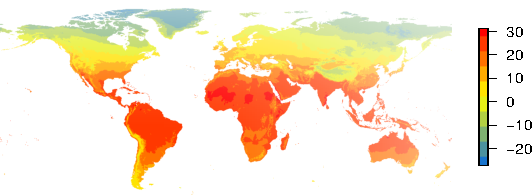
\includegraphics[width=1\linewidth]{figuresAz/AnmeanTempST.pdf}
\smallcitation{Worldclim data}

\end{frame}

\begin{frame}{Effects of temperature}

\begincols
 \column{0.48\textwidth} \centering
 Metabolic rate \par
 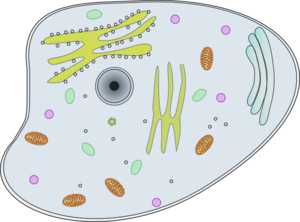
\includegraphics[width=0.4\linewidth]{figuresAz/cell.png}\par
 \vspace{1cm} \pause
 Biological rates (growth rate) \par
 
\includegraphics[width=0.5\linewidth]{figuresAz/fish_pop.pdf} \pause
 \hfill\column{0.48\textwidth} \centering
 Body-size \par
 
\includegraphics[width=0.6\linewidth]{figuresAz/size.pdf}\par
 \vspace{1cm} \pause
 Species distribution \par
 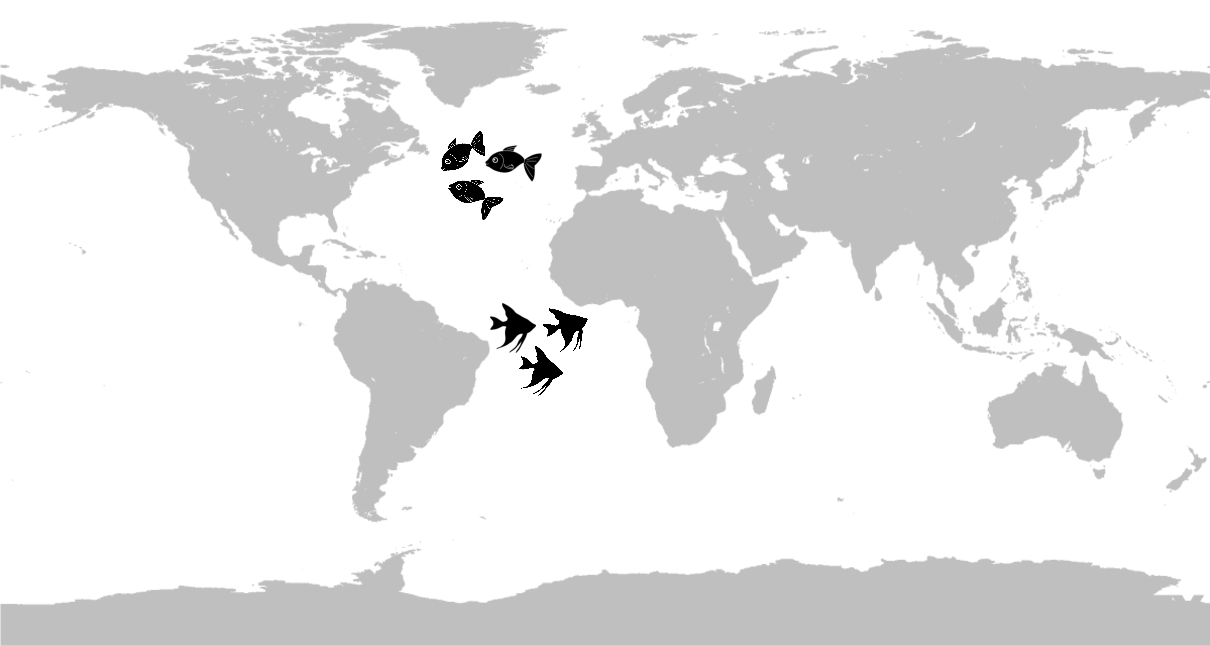
\includegraphics[width=0.8\linewidth]{figuresAz/world.pdf} \par

\stopcols

\end{frame}

\begin{frame}{Landscape-level effects of trophic interactions}

\centering
 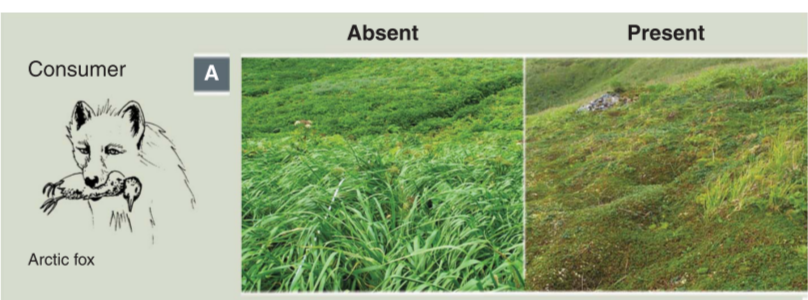
\includegraphics[width=0.7\linewidth]{figuresAz/estes2011.png}\par
\smallcitation{Estes \textit{et al} 2011}

\end{frame}

\begin{frame}{Effects of temperature on trophic regulation}

\centering
 % \documentclass[12pt,a4paper]{article}
%
% %%%%%%%%%%%%%%%%%%%%%%%%%%
% %% Packages %%
% % font
% \usepackage[T1]{fontenc}
% \usepackage[utf8]{inputenc}
% % language
% \usepackage[french, english]{babel}
%
% % marges, space...
% \usepackage[top=2.5cm, bottom=2.5cm, left=2.5cm, right=2.5cm]{geometry}
% \usepackage{setspace}
% \onehalfspacing
% \usepackage[font=footnotesize,labelfont=bf]{caption}
% \usepackage{subcaption}
%
% \usepackage{graphicx}
% \usepackage{float}
% \usepackage{pstool}
% \usepackage{multirow}
% \usepackage{booktabs,arydshln}
% % mathematics
% \usepackage{amsmath}
% \usepackage{textcomp}
%
% % TikZ
% \usepackage{tikz}
% 	\usetikzlibrary{arrows, plotmarks, decorations.markings}
% 	\tikzstyle{fleche} = [->,>=stealth,thick,rounded corners=4pt,line width=1pt]
% 	\tikzstyle{fleche2} = [->,>=stealth,thick,dashed,rounded corners=4pt,line width=2pt]
% 	\tikzstyle{fleche3} = [->,>=stealth,thick,rounded corners=4pt,line width=2pt]
% 	\usetikzlibrary{shadows}
% 	\usetikzlibrary{shadings,decorations.pathreplacing,angles,quotes}
%
%
% %%%%%%%%%%%%%%%%%%%%%%%%%%
%
% \begin{document}

%
% % FIGURE MODEL %%
% \begin{figure}[!h]
% \tikzset{
% 	invisible/.style={opacity=0},
% 	visible on/.style={alt={#1{}{invisible}}},
% 	alt/.code args={<#1>#2#3}{%
% 		\alt<#1>{\pgfkeysalso{#2}}{\pgfkeysalso{#3}} % \pgfkeysalso doesn't change the path
% 	},
% }

\begin{tikzpicture}[thick]
	\draw (4,6) circle (0.65);
	\node (C) at (4,6) {C};

	\draw (4,3) circle (0.65);
	\node (H) at (4,3) {H};

	\draw (4,0) circle (0.65);
	\node (P) at (4,0) {P};

	\node (T) at (0,3) {\textbf{\huge T}};

	\node (CH) at (4,5.2) {};
	\draw[fleche] (CH) -- (4,3.8);

	\node (HP) at (4,2.2) {};
	\draw[fleche] (HP) -- (4,0.8);

	\draw[fleche2]	(T) to node [midway] (H) {} (2.5,3);


\draw[decoration={brace,mirror,raise=5pt,amplitude=20pt},decorate]
	  (5.5,0) -- node[right=35pt, text width = 4cm] (FI) {Interaction strength} (5.5,6);



\end{tikzpicture}
% \end{figure}
%
% \end{document}
\par

\end{frame}

\begin{frame}{Effects of temperature on trophic regulation}

\centering
% \documentclass[12pt,a4paper]{article}
%
% %%%%%%%%%%%%%%%%%%%%%%%%%%
% %% Packages %%
% % font
% \usepackage[T1]{fontenc}
% \usepackage[utf8]{inputenc}
% % language
% \usepackage[french, english]{babel}
%
% % marges, space...
% \usepackage[top=2.5cm, bottom=2.5cm, left=2.5cm, right=2.5cm]{geometry}
% \usepackage{setspace}
% \onehalfspacing
% \usepackage[font=footnotesize,labelfont=bf]{caption}
% \usepackage{subcaption}
%
% \usepackage{graphicx}
% \usepackage{float}
% \usepackage{pstool}
% \usepackage{multirow}
% \usepackage{booktabs,arydshln}
% % mathematics
% \usepackage{amsmath}
% \usepackage{textcomp}
%
% % TikZ
% \usepackage{tikz}
% 	\usetikzlibrary{arrows, plotmarks, decorations.markings}
% 	\tikzstyle{fleche} = [->,>=stealth,thick,rounded corners=4pt,line width=1pt]
% 	\tikzstyle{fleche2} = [->,>=stealth,thick,dashed,rounded corners=4pt,line width=2pt]
% 	\tikzstyle{fleche3} = [->,>=stealth,thick,rounded corners=4pt,line width=2pt]
% 	\usetikzlibrary{shadows}
% 	\usetikzlibrary{shadings,decorations.pathreplacing,angles,quotes}
%
%
% %%%%%%%%%%%%%%%%%%%%%%%%%%
%
% \begin{document}

%
% % FIGURE MODEL %%
% \begin{figure}[!h]


\begin{tikzpicture}[thick]
	\draw (4,6) circle (0.65);
	\node (C) at (4,6) {C};

	\draw (4,3) circle (0.65);
	\node (H) at (4,3) {H};

	\draw (4,0) circle (0.65);
	\node (P) at (4,0) {P};

	\node (T) at (0,3) {\textbf{\huge T}};

	\node (CH) at (4,5.2) {};
	\draw[fleche3] (CH) -- (4,3.8);

	\node (HP) at (4,2.2) {};
	\draw[fleche3] (HP) -- (4,0.8);

	\draw[fleche2]	(T) to node [midway] (H) {} (2.5,3);


\draw[decoration={brace,mirror,raise=5pt,amplitude=20pt},decorate]
	  (5.5,0) -- node[right=35pt, text width = 4cm] (FI) {\textbf{Interaction strength}} (5.5,6);

\end{tikzpicture}
% \end{figure}
%
% \end{document}
\par
\smallcitation{Beveridge et al 2010, Kratina et al 2012, Shurin et al 2012}

\end{frame}

\section{Model}\label{model}

\begin{frame}{Tri-trophic model}

\begincols
 \column{0.48\textwidth} \centering
 
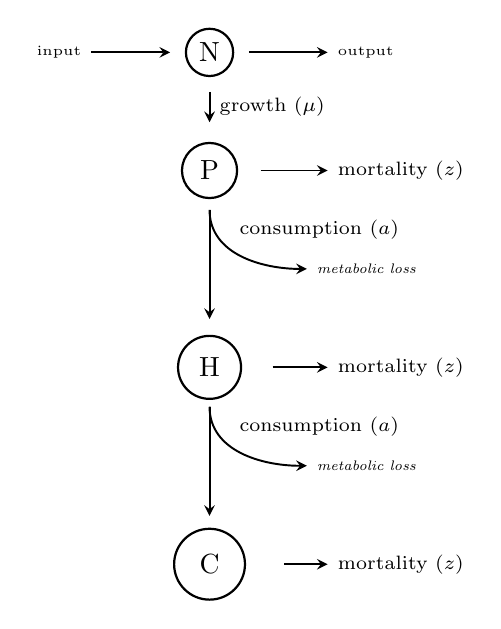
\begin{tikzpicture}[thick]
%% Les lettres, cercles et fl�ches verticales
	\draw (0,0) circle (0.45);
	\node (C) at (0,0) {C};

	\draw (0,2.5) circle (0.4);
	\node (H) at (0,2.5) {H};

	\draw (0,5) circle (0.35);
	\node (P) at (0,5) {P};

	\draw (0,6.5) circle (0.3);
	\node (N) at (0,6.5) {N};

	\node [above =0.1cm of C](C1) {};
	\node [above =0.1cm of H] (H1) {};
	\node [above =0.1cm of P] (P1) {};

	\draw[fleche] (0,2) -- (C1);
	\draw[fleche] (0,4.5) -- (H1);
	\draw[fleche] (0,6) to node [midway,right] {\scriptsize growth ($\mu$)} (P1);


%% in/out N
	\node[left] (in_N) at (-1.5,6.5) {\tiny input};
	\draw[fleche] (in_N) -- (-0.5,6.5);

	\node[right] (out_N) at (1.5,6.5) {\tiny output};
	\draw[fleche] (0.5,6.5) -- (out_N);

%% in/out P
	\node[right] (out_P) at (1.5,5) {\scriptsize mortality ($z$)};
	\draw[fleche] (0.65,5) -- (out_P);

%% out H
	\node[right] (out_H) at (1.5,2.5) {\scriptsize mortality ($z$)};
	\draw[fleche] (0.8,2.5) -- (out_H);

%% out C
	\node[right] (out_C) at (1.5,0) {\scriptsize mortality ($z$)};
	\draw[fleche] (0.95,0) -- (out_C);

%% loss
	\node (loss2) at (2,3.75) {\textit{\tiny metabolic loss}};
	\draw[fleche] (0,4.5) to[out=-90, in=-180] (loss2);

	\node (loss1) at (2,1.25) {\textit{\tiny metabolic loss}};
	\draw[fleche] (0,2) to[out=-90, in=-180] (loss1);

%% Equations conso (bottom)
	\node (inv1) at (0.25,4.5) {};
	\node[below right] at (inv1) {\scriptsize consumption ($a$)};

	\node (inv2) at (0.25,3) {};
	\node[above right] at (inv2) {};

	\node (inv3) at (0.25,2) {};
	\node[below right] at (inv3) {\scriptsize consumption ($a$)};

	\node (inv4) at (0.25,0.5) {};
	\node[above right] at (inv4) {};

\end{tikzpicture}
\par
 \hfill\column{0.48\textwidth}

\begin{description}
\tightlist
\item[\(\mu\)]
growth rate
\item[\(a\)]
attack rate
\item[\(z\)]
mortality rate
\end{description}

\stopcols

\end{frame}

\begin{frame}{Temperature dependence of organisms' biological rates}

\begincols
\column{0.48\textwidth} \centering
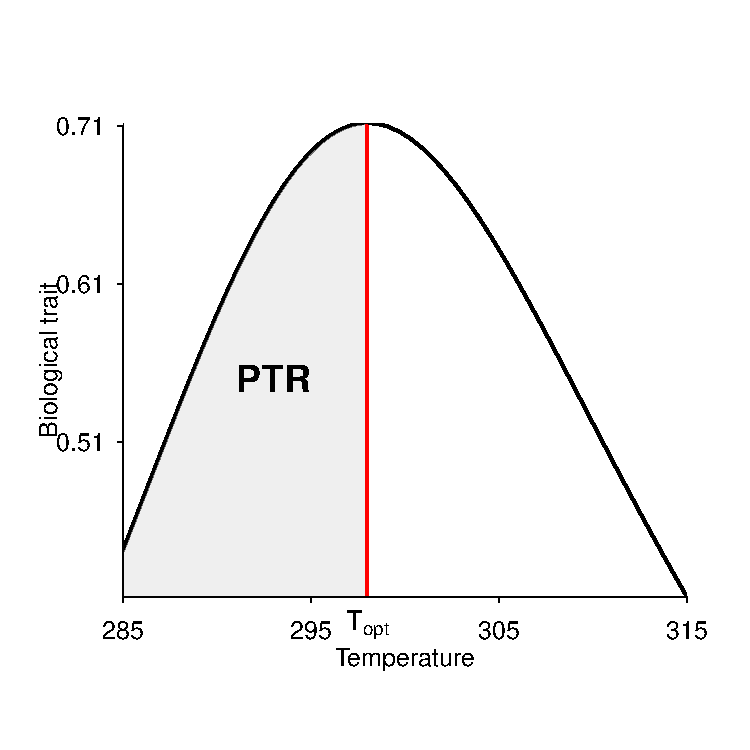
\includegraphics[width=1\linewidth]{figuresAz/MTE.pdf}

\hfill\column{0.48\textwidth}

\[
    r(T)= r_0 \textbf{m}^{\beta} exp^{\biggl(-\dfrac{\textbf{E}}{k\textbf{T}}\biggr)}\mathlarger{L}(T)
\]

~

\begin{description}
\tightlist
\item[\(r(T)\)]
biological rate
\item[\(m\)]
body-mass
\item[\(E\)]
activation energy
\item[\(T\)]
temperature
\item[\(L(T)\)]
decreasing phase
\item[\(\beta\), \(r_0\), \(k\)]
constants
\end{description}

\stopcols
\smallcitation{Gillooly et al 2001, Brown et al 2004, Savage et al 2004, Pawar et al 2015}

\end{frame}

\section{Direct and indirect effects of temperature on trophic
regulation}\label{direct-and-indirect-effects-of-temperature-on-trophic-regulation}

\begin{frame}{Interaction strength measures}

\centering
 % \documentclass[12pt,a4paper]{article}
%
% %%%%%%%%%%%%%%%%%%%%%%%%%%
% %% Packages %%
% % font
% \usepackage[T1]{fontenc}
% \usepackage[utf8]{inputenc}
% % language
% \usepackage[french, english]{babel}
%
% % marges, space...
% \usepackage[top=2.5cm, bottom=2.5cm, left=2.5cm, right=2.5cm]{geometry}
% \usepackage{setspace}
% \onehalfspacing
% \usepackage[font=footnotesize,labelfont=bf]{caption}
% \usepackage{subcaption}
%
% \usepackage{graphicx}
% \usepackage{float}
% \usepackage{pstool}
% \usepackage{multirow}
% \usepackage{booktabs,arydshln}
% % mathematics
% \usepackage{amsmath}
% \usepackage{textcomp}
%
% % TikZ
% \usepackage{tikz}
% 	\usetikzlibrary{arrows, plotmarks, decorations.markings}
% 	\tikzstyle{fleche} = [->,>=stealth,thick,rounded corners=4pt,line width=1pt]
% 	\tikzstyle{fleche2} = [->,>=stealth,thick,dashed,rounded corners=4pt,line width=2pt]
% 	\tikzstyle{fleche3} = [->,>=stealth,thick,rounded corners=4pt,line width=2pt]
% 	\usetikzlibrary{shadows}
% 	\usetikzlibrary{shadings,decorations.pathreplacing,angles,quotes}
%
%
% %%%%%%%%%%%%%%%%%%%%%%%%%%
%
% \begin{document}
%
%
% % FIGURE MODEL %%
% \begin{figure}[!h]


\begin{tikzpicture}[thick]

	\draw (-1,3) circle (0.65);
	\node (H0) at (-1,3) {$H$};
	\node [above =0.5cm of H0] (ISpc) {Per capita};

	\draw (-1,0) circle (0.65);
	\node (PH0) at (-1,0) {$P_H$};

	\node (lPH0) at (-1,2.2) {};
	\draw[fleche] (lPH0) -- (-1,0.8) node [right, midway] {$a_{\textsc{\tiny ph}}$};

	\draw[trait2] (1,4) -- (1,-1);

		\draw (3,3) circle (0.65);
		\node (H1) at (3,3) {$H^*$};
		\node [above =0.5cm of H1] (ISpop) {Per population};

		\draw (3,0) circle (0.65);
		\node (PH1) at (3,0) {$P^*_H$};

		\node (lPH1) at (3,2.2) {};
		\draw[fleche] (lPH1) -- (3,0.8) node [right, midway] {$a_{\textsc{\tiny ph}} H^*$};

		\draw[trait2] (5.5,4) -- (5.5,-1);

	\draw (9,3) circle (0.65);
	\node (H2) at (9,3) {$H^*$};
	\node [above left =0.5cm and 0.5 cm of H2] (ISnet) {Net};


	\draw (9,0) circle (0.65);
	\node (PH2) at (9,0) {$P^*_H$};

	\draw (7,0) circle (0.65);
	\node (P02) at (7,0) {$P^*_0$};

	\node (lPH2) at (9,2.2) {};
	\draw[fleche] (lPH2) -- (9,0.8);

\draw[decoration={brace,mirror,raise=5pt,amplitude=20pt},decorate]
	  (6,-1) -- node[below=35pt] (D) {Density ratio $\dfrac{P^*_0}{P^*_H}$} (10,-1);

\end{tikzpicture}
% \end{figure}
%
% \end{document}
\par

\end{frame}

\begin{frame}{Direct and indirect effects of temperature}

Direct effect on biological traits \par

\includegraphics[width=0.2\linewidth]{figuresAz/fish_pop.pdf} \par
\vspace{1cm}

Indirect effect through decreasing body-size \par


\includegraphics[width=0.2\linewidth]{figuresAz/size.pdf}

\end{frame}

\section{Results}\label{results}

\begin{frame}{Direct effect of temperature on biological traits}

\centering

\includegraphics[width=0.4\linewidth]{figuresAz/fish_pop.pdf} \par

\end{frame}

\begin{frame}{Temperature dependence of interaction strength measures
are consistent}

\centering
Effect of herbivore on primary producers \vspace{1cm}

\begincols
 \column{.33\textwidth} \centering
 Per capita 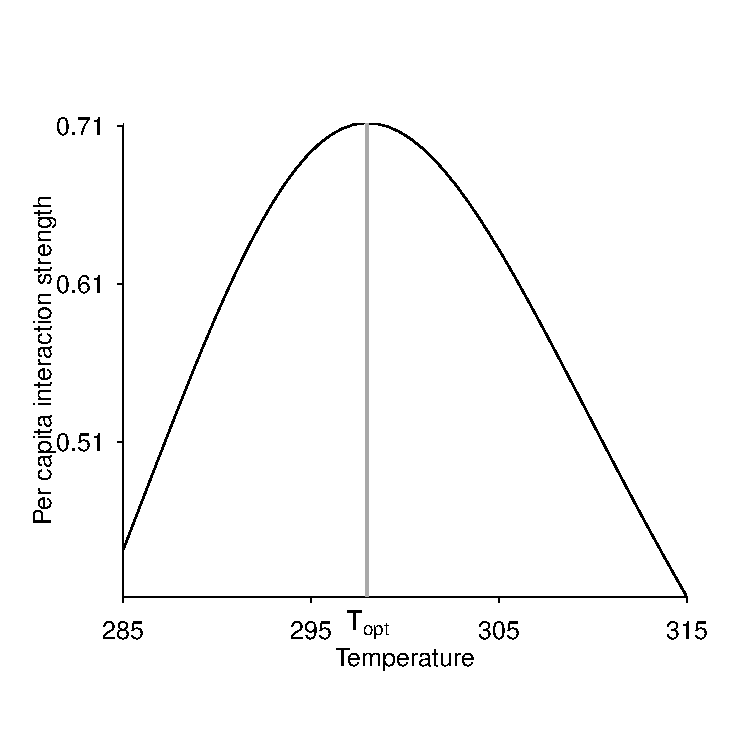
\includegraphics[width=1.1\linewidth]{figuresAz/ISpc.pdf}
\column{.33\textwidth} \centering
 Per population
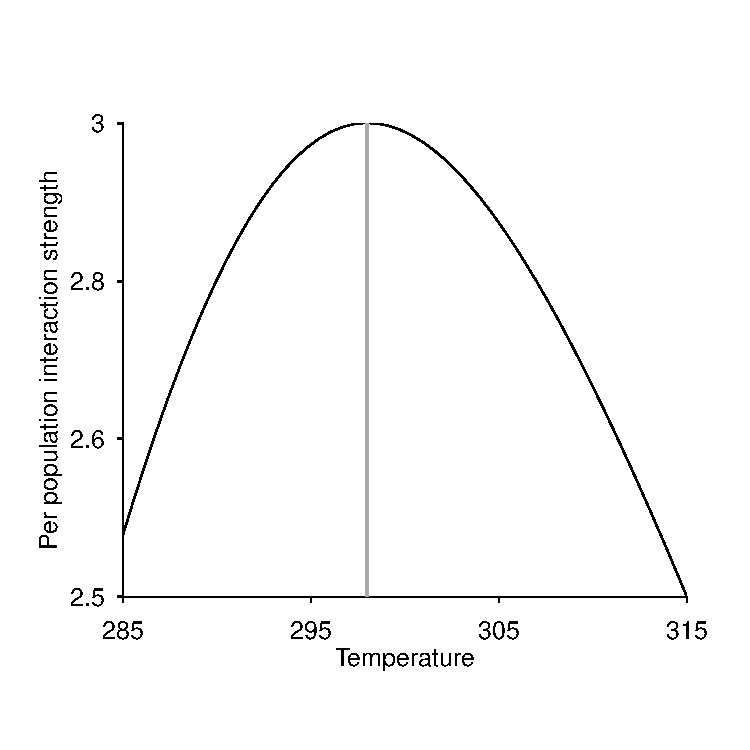
\includegraphics[width=1.1\linewidth]{figuresAz/ISpop.pdf}

\column{.33\textwidth} \centering
 Net 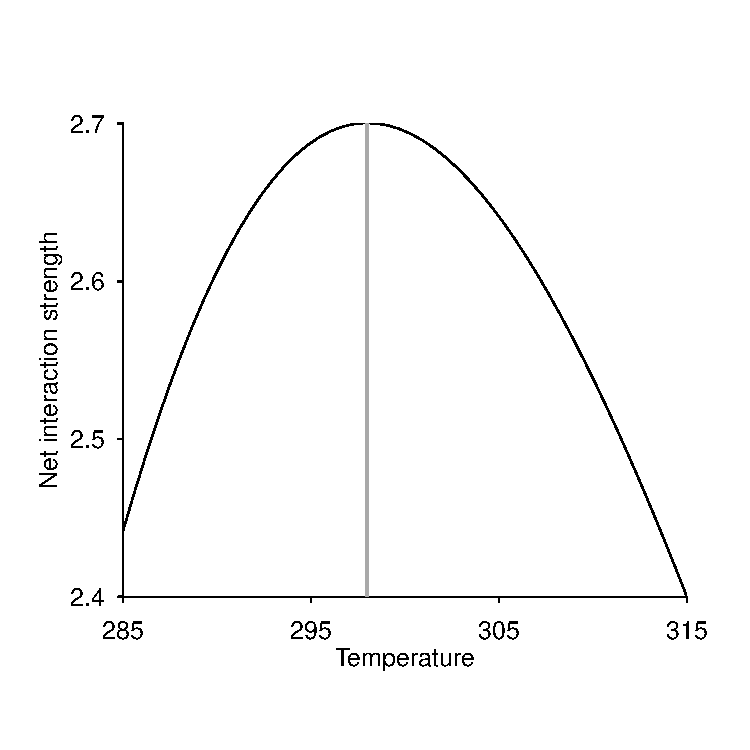
\includegraphics[width=1.1\linewidth]{figuresAz/NetIS.pdf}

\stopcols

\end{frame}

\begin{frame}{Heterogeneous dependencies}

\centering
Effect of carnivores on herbivores ~

\begin{longtable}[c]{@{}lcc@{}}
\toprule
Fixed parameters & IS per population & IS net\tabularnewline
\midrule
\endhead
\(\emptyset\) & \(\cap\) & \(\cap\)\tabularnewline
\(a_{hc}\) & \(\cap\) & \(\textcolor{red}{\cup}\)\tabularnewline
\(a_{ph}\), \(a_{hc}\) & \(\textcolor{red}{\cup}\) &
\(\textcolor{red}{\cup}\)\tabularnewline
H: \(a_{ph}\), \(z_h\) & \(\textcolor{red}{\cup}\) &
\(\cap\)\tabularnewline
C: \(a_{hc}\), \(z_c\) & \(\cap\) &
\(\textcolor{red}{\cup}\)\tabularnewline
\bottomrule
\end{longtable}

\begin{description}
\tightlist
\item[\(a\)]
attack rate
\item[\(z\)]
mortality rate
\end{description}

\end{frame}

\begin{frame}{Indirect effect of temperature through decreasing
body-size}

\centering

\includegraphics[width=0.7\linewidth]{figuresAz/size.pdf}

\end{frame}

\begin{frame}{Indirect effect of temperature through decreasing
body-size}

\centering
Effect of carnivores on herbivores \vspace{1cm}

\begincols
 \column{.33\textwidth} \centering
Per capita 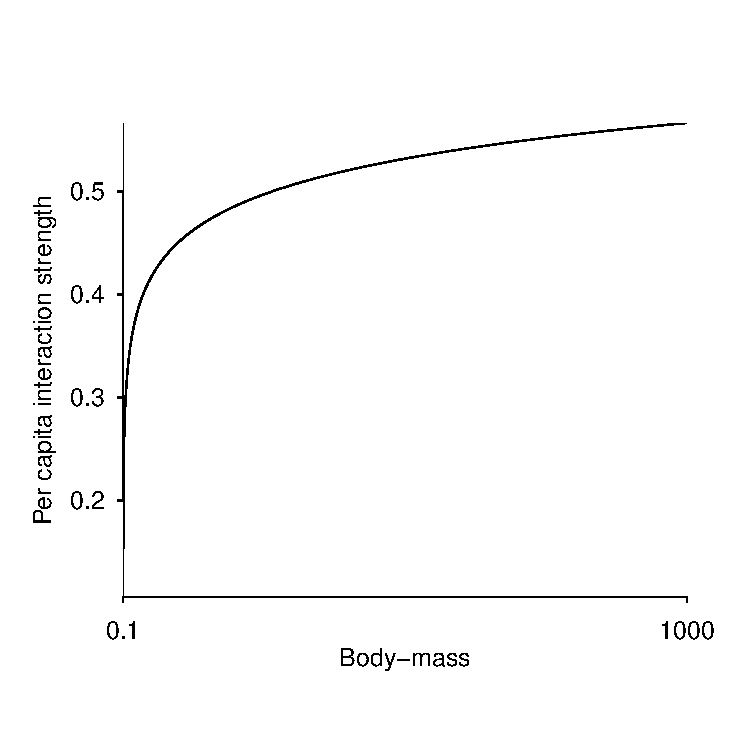
\includegraphics[width=1.1\linewidth]{figuresAz/ISpcBS.pdf}
\column{.33\textwidth} \pause
\centering
Per population
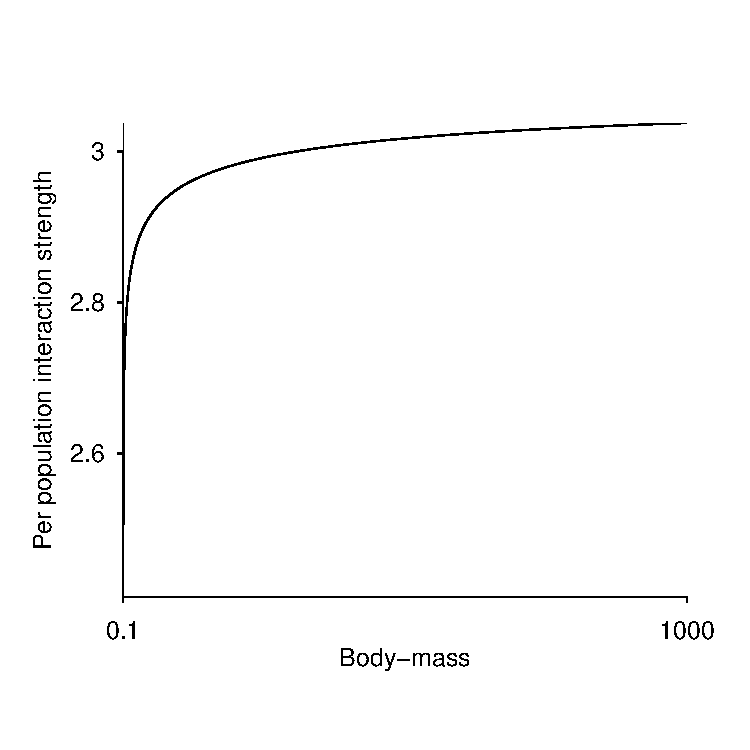
\includegraphics[width=1.1\linewidth]{figuresAz/ISpopBS.pdf}

\column{.33\textwidth} \pause
\centering
Net 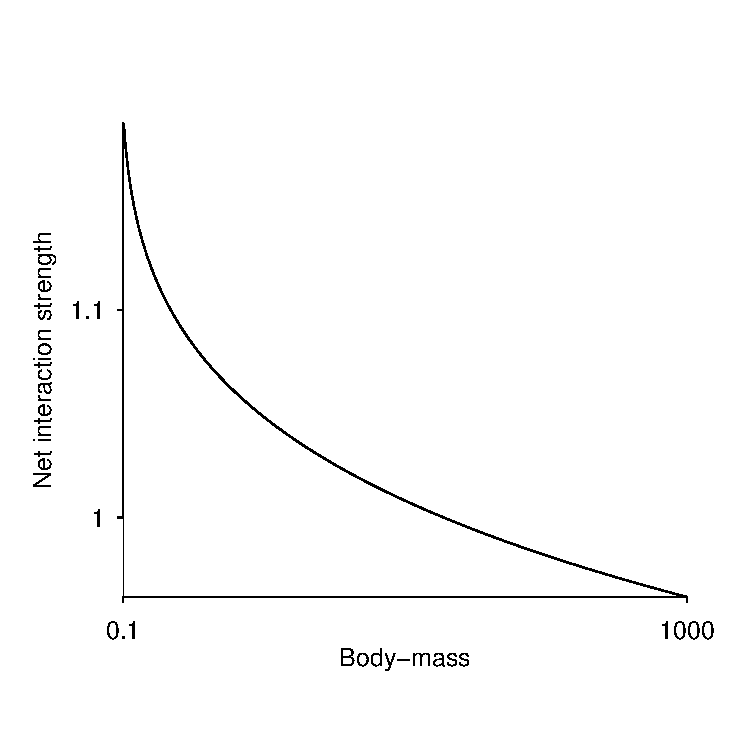
\includegraphics[width=1.1\linewidth]{figuresAz/ISnetBS.pdf}

\stopcols

\end{frame}

\begin{frame}{Effect of temperature on interaction strength through
biological traits}

\centering

\includegraphics[width=0.3\linewidth]{figuresAz/fish_pop.pdf} \par

\begin{itemize}
\tightlist
\item
  Temperature dependence of different interaction strength measures are
  consistent
\item
  Heterogeneous dependencies: variations according to which parameters
  are temperature dependent
\end{itemize}

\end{frame}

\begin{frame}{Indirect effect of temperature on interaction strength}

\centering
 
\includegraphics[width=0.3\linewidth]{figuresAz/size.pdf} \par

\begin{itemize}
\tightlist
\item
  Temperature can indirectly decrease or increase interaction strength
\item
  The indirect effect of temperature on trophic regulation through
  decreasing body-size may enhance or decrease its direct effect on
  biological traits
\end{itemize}

\end{frame}

\begin{frame}{Various effects of temperature on interaction strength}

\centering
Temperature has numerous and potentially conflicting effects on
interaction strength: \par
\vspace{1cm} developping a framework that integrates various effects of
temperature on interaction strength is key in understanding food web
dynamics

\end{frame}

\begin{frame}{Merci de votre attention}

\end{frame}

\begin{frame}[plain]
  \begin{picture}(0,0)
    \put(-28.5,-175){%
      \pgfuseimage{titlebackground}
    }
  \end{picture}
\end{frame}

\end{document}
